% prelab2
\documentclass{IEEEtran}
\usepackage{booktabs}
\usepackage{graphicx}
\usepackage{fancyhdr}
\usepackage{framed}
\pagestyle{fancy}
\lhead{}
\chead{}
\rhead{}
\lfoot{}
\cfoot{}
\rfoot{\thepage}
\title{Prelab 2 Amplifiers}
\author{Group 8: Muhan Li \and Man Sun \and Mingxiao An \\ EE233 Circuit Theory}
\IEEEaftertitletext{\centering \fontsize{11}{11}\textsc{Department of Electrical Engineering, University of Washington, Seattle, WA, 98195}}

\begin{document}
	\maketitle
	\section{\textbf{Prelab\#1}}
	The typical values of parameters of \textit{LM148} are shown in table[\ref{tab:pl1}], figure[\ref{fig:101}], and figure[\ref{fig:102}].
	\begin{table}[!htbp]
		\centering
		\caption{The typical values of parameters}
		\begin{tabular}{lcl}
			\toprule
			Parameter & value & \\
			\midrule
			Power supplies & $\pm22\mathrm{V}$ & \\
			Input resistance & $2.5\mathrm{M\Omega}$ & \\
			Slew rate & $0.5\mathrm{V}/\mathrm{s}$& \\
			\bottomrule
		\end{tabular}
		\label{tab:pl1}
	\end{table}
	\begin{figure}[!htbp]
		\centering
		\begin{framed}
			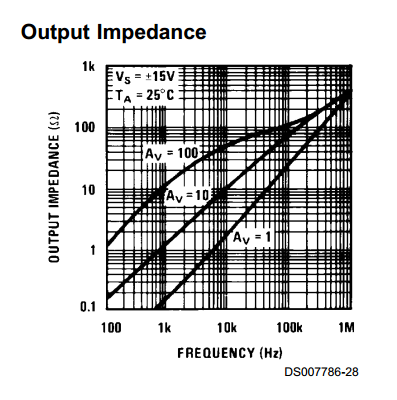
\includegraphics[width=\linewidth]{images/1_1.PNG}
			\caption{Output impedance}
		\end{framed}
		\label{fig:101}
	\end{figure}
	\begin{figure}[!htbp]
		\centering
		\begin{framed}
			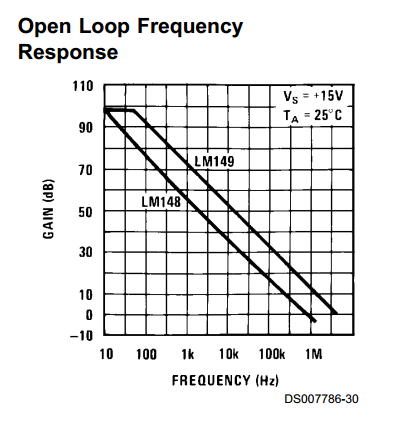
\includegraphics[width=\linewidth]{images/1_2.PNG}
			\caption{Open-loop voltage gain}
		\end{framed}
		\label{fig:102}
	\end{figure}
	\section{\textbf{Prelab\#2}}
\end{document}

